\section{Reference value \label{sec:reference}}

Our benchmarking framework will compute the context switching time but we need to know how well or how bad our framework performs.
To assess the performance of our measurements, we first need to compute the real context switching time.
This real context switching time will be our reference value.

\subsection{Simple application}
In order to experiment and test our benchmarking framework, we need to have a simple application on every tested RTOS.

The application contains two indentical tasks.
The tasks wait for 1ms in the foreground and then goes to the background letting the scheduler runs the next task.
The tasks run in an infinite loop.

\subsubsection{Implementation in Contiki}
The source code of one of the two tasks is shown in the listing \ref{lst:simple-task-code}.
It uses the \texttt{clock\_delay\_usec()} call to make the task wait for 1ms.
Finally, we use the \texttt{PROCESS\_PAUSE()} macro to pause the task and let the other task do its iteration.

\begin{lstlisting}[style=CStyle, float, label={lst:simple-task-code}, caption={Source code of a task implemented in Contiki for the simple application}]
PROCESS_THREAD(task, ev, data)
{
    PROCESS_BEGIN();

    while (1)
    {
        clock_delay_usec(1000);
        PROCESS_PAUSE();
    }

    PROCESS_END();
}
\end{lstlisting}

\subsubsection{Implementation in RIOT}
The source code of on of the two tasks is shown in the listing \ref{lst:simple-task-code-riot}.
We can not use the \texttt{xtimer\_usleep()} method as it will lead to a context switch.
Instead, we used a for loop.
The \texttt{thread\_yield()} call will perfom a context switch and let the other task run on iteration.

\begin{lstlisting}[style=CStyle, float, label={lst:simple-task-code-riot}, caption={Source code of a task implemented in RIOT for the simple application}]
void *threadA(void *arg)
{
    (void)arg;

    while (1)
    {
        for(int i = 0; i < 1000; i++) {}
        thread_yield();
    }
    return NULL;
}
\end{lstlisting}


\subsection{Methodology}

In order to compute the real context switching time, we used an oscilloscope and two GPIOs.
Each task of our simple application is responsible of one GPIO.
Every time a task is run and goes to the foreground, it sets its GPIO up.
Once the task is finished and goes to the background, it resets its GPIO down.

With the oscilloscope, we can mesure the voltage of the two GPIOs and compute the real context switching time from those measurements.
The figure \ref{fig:real-context-switching-time-measurement} shows the different steps of our methodology.
On this schema, the execution time of the two tasks are represented above the voltage measurements of the two GPIOs.
The context switching time happens between the execution of the two tasks and is bordered with dotted lines.

\begin{figure}[!ht]
  \centering
  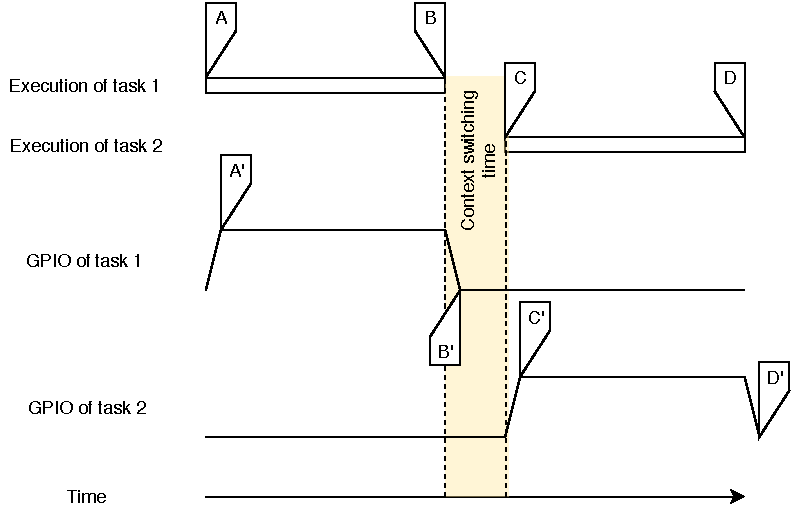
\includegraphics[scale=1]{assets/real-context-switching-time-measurement.pdf}
  \caption{\label{fig:real-context-switching-time-measurement}Steps in the methodology to compute the real context switching time}
\end{figure}

The steps are the following.
The first task sets up its GPIO on step A.
The GPIO is in high position few nano seconds later on step A'.
Once the first task is over, it resets its GPIO on step B which goes in low position on step B'.
In the same way, the second task set up its GPIO on step C which goes in high position on step C' few nano seconds later and reset it on step D which goes in low position on step D'.
The oscilloscope measures the context switching time between the step B' and the step C'.
The time for the GPIOs to rise up or down are around 10 nano seconds and can be omitted.


\subsection{Measurement setup}

The oscilloscope used for the measurement was the \href{https://www.tek.com/oscilloscope/mso56}{Tektronix MSO 56} available at the Welcome Lab at UCLouvain.
We used two channels to measure the voltage of the two GPIOs used by the application.
The interface of the oscilloscope, shown in the figure \ref{fig:oscilloscope-interface}, allows us to directly see in real-time our measurements.
A table resume the measurements displayed in the graph below while we can check the voltage of our two GPIOs in the bottom-right window.
Once we have retrieved 1000 measurements, we export our data in a flash thumb.

\begin{figure}[!ht]
    \centering
    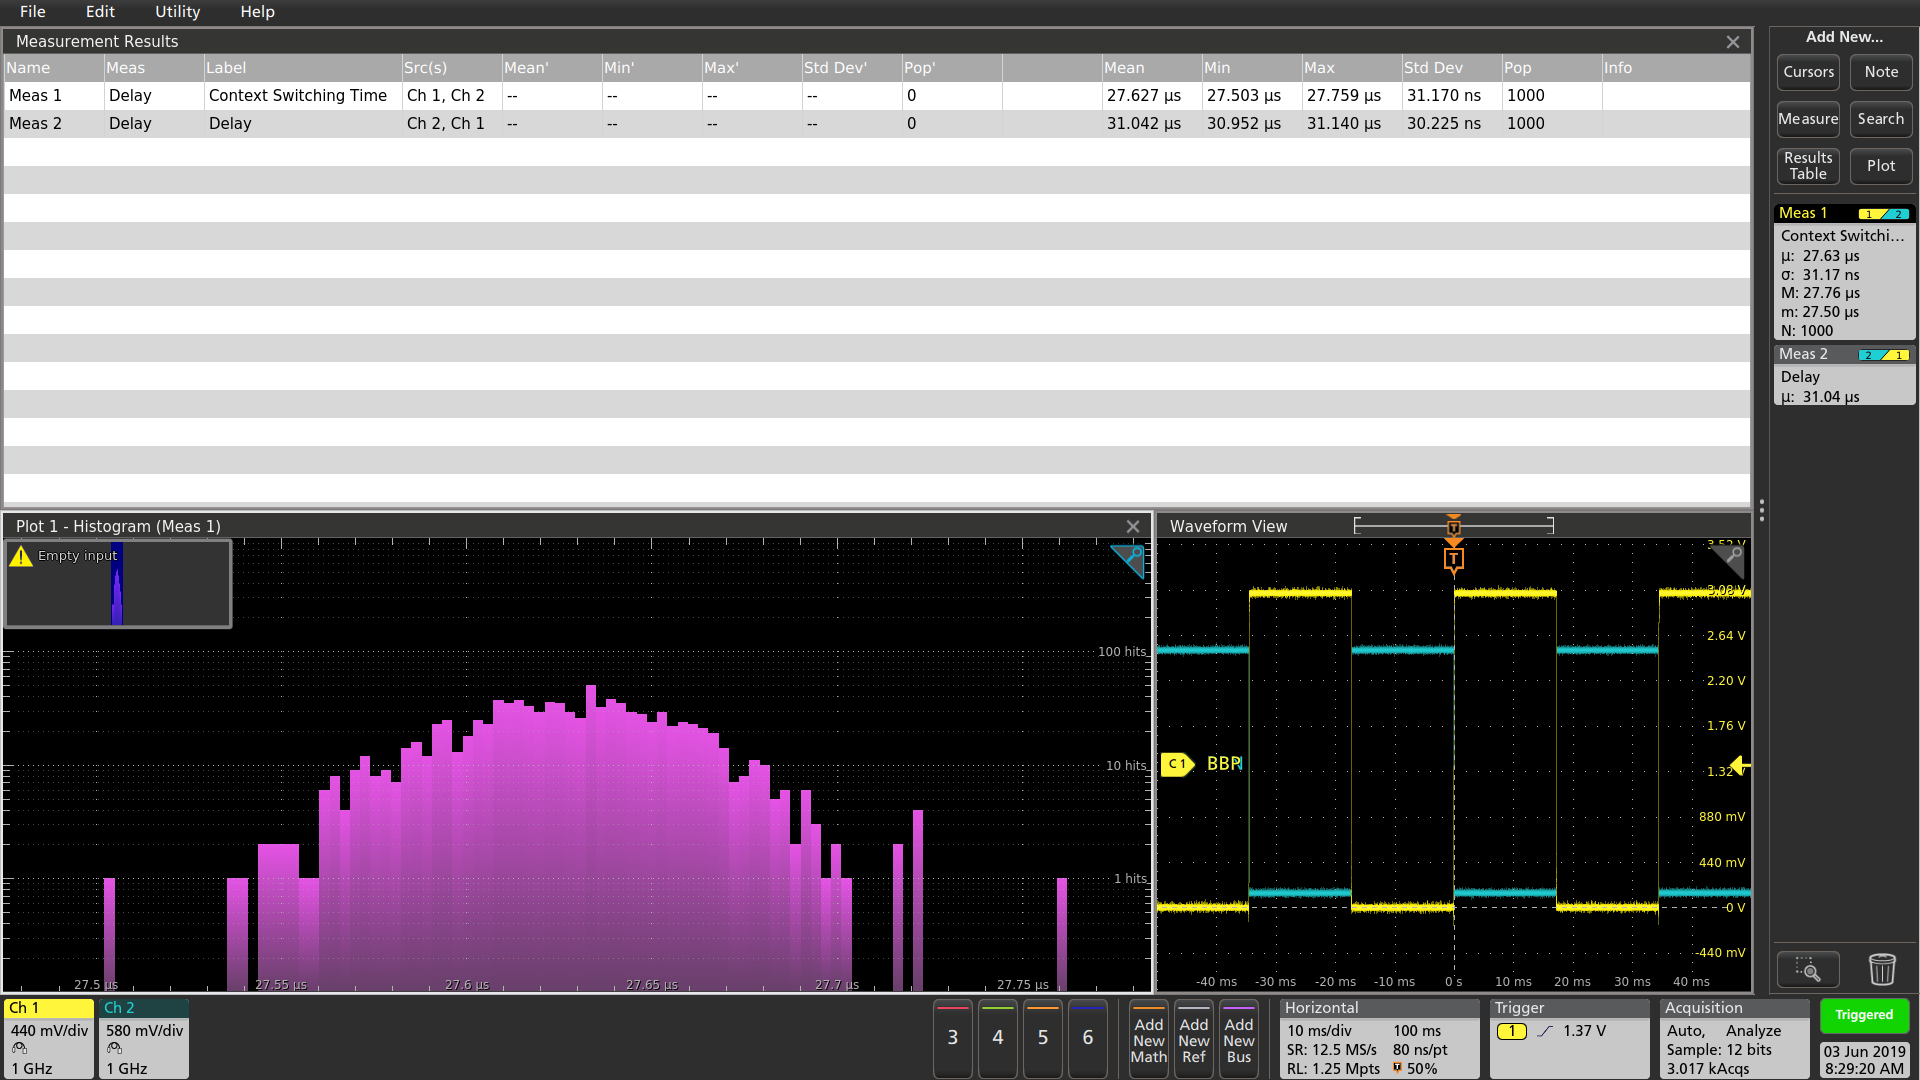
\includegraphics[scale=0.25]{assets/oscilloscope-interface.png}
    \caption{Interface of the oscilloscope\label{fig:oscilloscope-interface}}
\end{figure}

We updated our simple task by adding GPIO calls in order for the oscilloscope to detect it.
The task will set up a GPIO, wait for 1ms, and then clear the GPIO.
The two tasks use different GPIO in order to differenciate them with the oscilloscope.

\subsubsection{Implementation in Contiki}
The source code of the updated task is shown in the listing \ref{lst:gpio-task-code}.
\texttt{GPIO\_SET\_PIN()} and \texttt{GPIO\_CLR\_PIN()} are used to respectively set and clear the GPIO used by the task.

\begin{lstlisting}[style=CStyle, float, label={lst:gpio-task-code}, caption={Source code of the task with GPIO calls}]
  PROCESS_THREAD(task, ev, data)
  {
      PROCESS_BEGIN();
  
      while (1)
      {
          GPIO_SET_PIN(
              GPIO_PORT_TO_BASE(GPIO_C_NUM), 
              GPIO_PIN_MASK(3));

          clock_delay_usec(1000);

          GPIO_CLR_PIN(
              GPIO_PORT_TO_BASE(GPIO_C_NUM), 
              GPIO_PIN_MASK(3));

          PROCESS_PAUSE();
      }
  
      PROCESS_END();
  }
\end{lstlisting}

\subsubsection{Implemetation in RIOT}
The source code of the updated task is shown in the listing \ref{lst:gpio-task-code-riot}.
\texttt{gpio\_set()} and \texttt{gpio\_clear()} are used to respectively set and clear the GPIO used by the task.

\begin{lstlisting}[style=CStyle, float, label={lst:gpio-task-code-riot}, caption={Source code of a task implemented in RIOT for the simple application}]
    void *thread(void *arg)
    {
        (void)arg;
    
        while (1)
        {
            gpio_set(GPIO_PIN(PORT_C, 2));

            for(int i = 0; i < 1000; i++) {}

            gpio_clear(GPIO_PIN(PORT_C, 2));

            thread_yield();
        }
        return NULL;
    }
    \end{lstlisting}

\subsubsection{Boards used}

To perform our measurements, we have used two devices from Zolertia.
The \href{https://github.com/Zolertia/Resources/wiki/RE-Mote}{RE-Mote} and the \href{https://github.com/Zolertia/Resources/wiki/The-Z1-mote}{Z1}.
The CPU of the RE-Mote is a \href{https://developer.arm.com/ip-products/processors/cortex-m/cortex-m3}{ARM Cortex-M3} 32 MHz clock speed with 512 KB flash and 32 KB RAM.
The Z1 have a \href{http://www.ti.com/product/MSP430F2617}{MSP430F2617} 16 MHz clock speed with 92KB flash and a 8KB RAM.

With those specifications, the Zolertia RE-Mote categorizes itself as a Class 2 device and the Zolertia Z1 as a Class 1 device.
Moreover, both Contiki and RIOT support those boards.

\begin{figure}[!ht]
    \begin{minipage}{.45\textwidth}
        \centering
        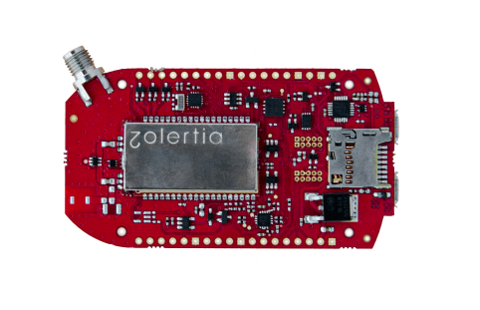
\includegraphics[scale=.5]{assets/remote.png}
        \caption{Zolerta RE-Mote board}
    \end{minipage}\hfill
    \begin{minipage}{.45\textwidth}        
        \centering
        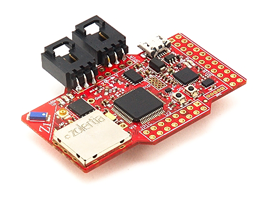
\includegraphics[scale=2.5]{assets/z1.png}
        \caption{Zolerta Z1 board}
    \end{minipage}
\end{figure}

\subsection{Measurement results\label{sec:ref-measurements}}

In the end, we have four differents reference values.
One for each board and for each RTOS.
The results are divided by boards and the measurements from Contiki are compared side-by-side with the measurements from RIOT for more clarity.

\subsubsection{RE-Mote measurements}
With the RE-Mote board, we have measured an average context switching time of $18.505\mu s$ for Contiki and $12.626 \mu s$ for RIOT.
The table \ref{tab:reference-value-remote} shows the statistics of the measurements.

\begin{table}[!ht]
  \centering
  \begin{tabular}{l|c|c}
       & Contiki & RIOT \\ \hline
  Mean ($\mu$s) & 18.505 & 12.626 \\
  Min  ($\mu$s) & 14.312 & 12.549 \\
  Max  ($\mu$s) & 72.753   & 12.656
  \end{tabular}
  \caption{Reference value for Contiki and RIOT on the RE-Mote}
  \label{tab:reference-value-remote}
  \end{table}

The figure \ref{fig:reference-value-contiki-remote} and the figure \ref{fig:reference-value-riot-remote} show the distribution of the reference value with the RE-Mote board.
Note that the y-axis is logarithmic.
For the reference value of Contiki, we can see that the majority of the measurements is around $14 \mu s$.
Some measurements are above $35 \mu s$ with extrema around $70 \mu s$.
For RIOT, we find two distributions.
One around $12.56\mu s$ and the other around $12.64\mu s$.

\begin{figure}[!ht]
    % \begin{minipage}{.45\textwidth}
        \centering
        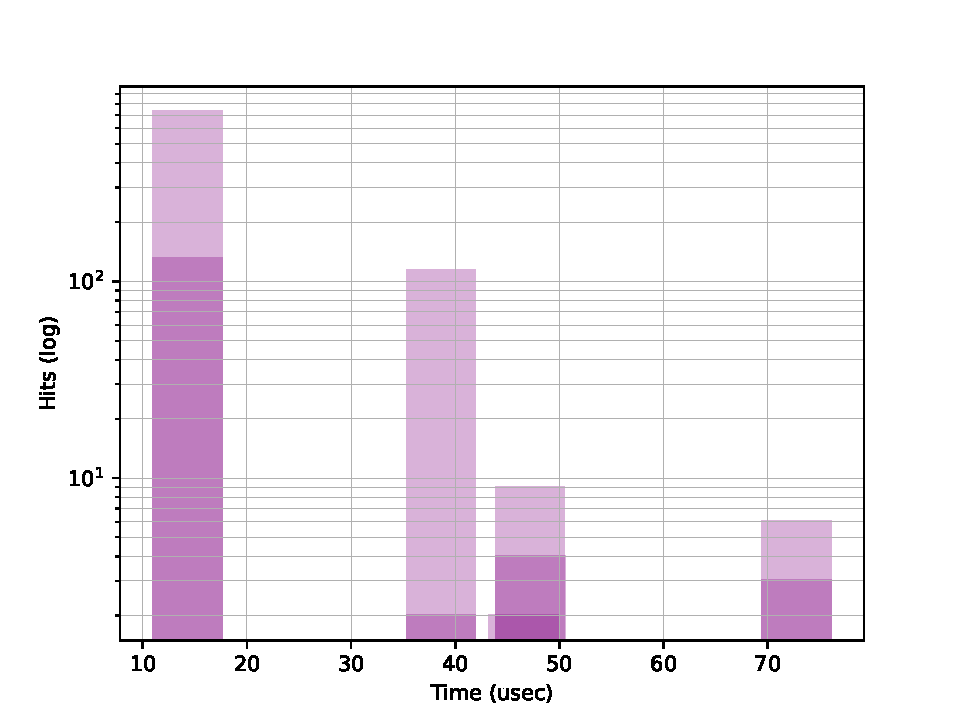
\includegraphics[scale=.7]{assets/reference-value-contiki-remote.pdf}
        \caption{Reference measurements distribution with Contiki on the RE-Mote board\label{fig:reference-value-contiki-remote}}
    % \end{minipage}\hfill
    % \begin{minipage}{.45\textwidth}        
        \centering
        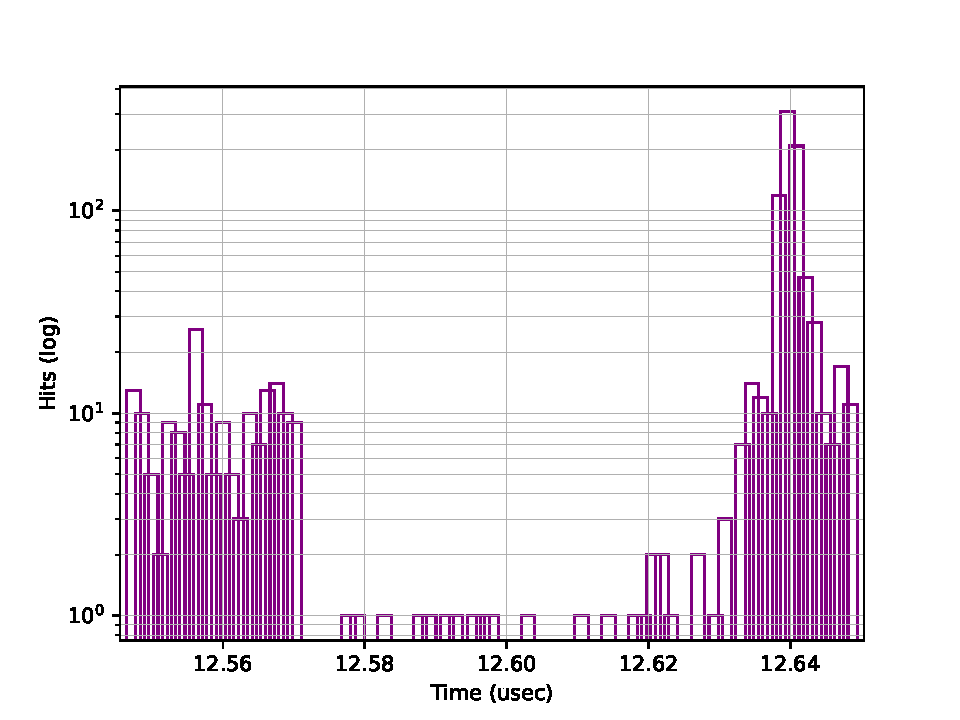
\includegraphics[scale=.7]{assets/reference-value-riot-remote.pdf}
        \caption{Reference measurements distribution with RIOT on the RE-Mote board\label{fig:reference-value-riot-remote}}
    % \end{minipage}
\end{figure}

\subsubsection{Z1 measurements}
With the Z1 board, we have measured an higher context switching time than with the RE-Mote board. The average context switching time for Contiki is $54.99\mu s$ and $30.6971 \mu s$ for RIOT.
It is not a surprise that the RE-Mote board have a smallest context switching time than the Z1 board as the latter is a Class-1 device while the former is a Class-2 device.
The table \ref{tab:reference-value-z1} shows the statistics of the measurements made with the Z1 board.

\begin{table}[!ht]
  \centering
  \begin{tabular}{l|c|c}
       & Contiki & RIOT OS \\ \hline
  Mean ($\mu$s) & 54.99   & 30.6971 \\
  Min  ($\mu$s) & 32.5625 & 30.5312 \\
  Max  ($\mu$s) & 314.5   & 30.8437
  \end{tabular}
  \caption{Reference value for Contiki and RIOT OS on the Z1}
  \label{tab:reference-value-z1}
  \end{table}

The figure \ref{fig:reference-value-contiki-z1} and the figure \ref{fig:reference-value-riot-z1} show the distribution of the reference value with the Z1 board.
Note that the y-axis is logarithmic.
This time, RIOT have a strong distribution around $27.625\mu s$.
For Contiki, in the other hand, we have the majority of our measurements around $32\mu s$ but some measurements are above $100 \mu s$.

\begin{figure}[!ht]
    % \begin{minipage}{.45\textwidth}
        \centering
        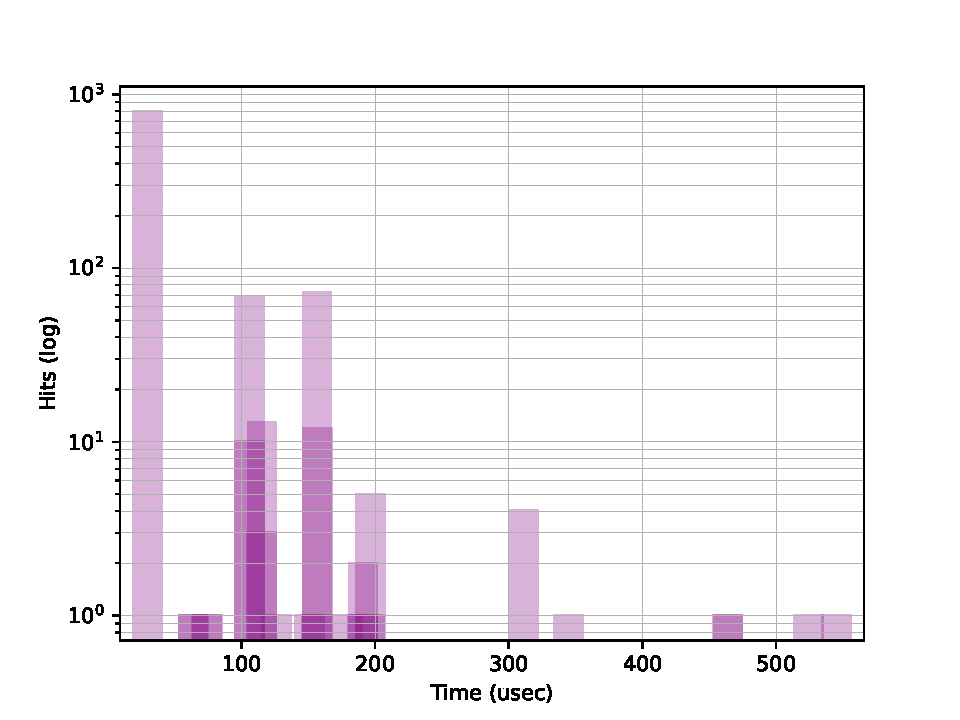
\includegraphics[scale=.7]{assets/reference-value-contiki-z1.pdf}
        \caption{Reference measurements distribution with Contiki on the Z1 board\label{fig:reference-value-contiki-z1}}
    % \end{minipage}\hfill
    % \begin{minipage}{.45\textwidth}        
        \centering
        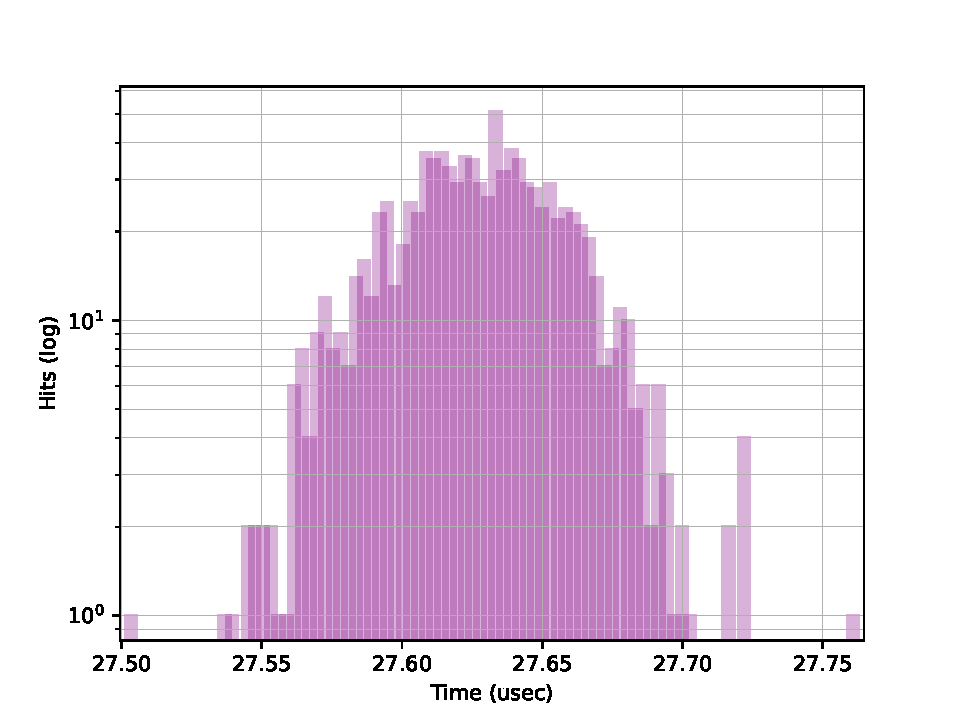
\includegraphics[scale=.7]{assets/reference-value-riot-z1.pdf}
        \caption{Reference measurements distribution with RIOT on the Z1 board\label{fig:reference-value-riot-z1}}
    % \end{minipage}
\end{figure}

\subsubsection{Resume}
The table \ref{tab:reference-values-resume} resume our reference values with the two boards, the RE-Mote and the Z1, and the two RTOS, Contiki and RIOT.

\begin{table}[!ht]
  \centering
  \begin{tabular}{l|c|c}
                   & Contiki  & RIOT    \\ \hline
  RE-Mote ($\mu$s) & 18.505  & 12.626   \\
  Z1 ($\mu$s)      & 55.077   & 27.699
  \end{tabular}
  \caption{Resume of the reference values}
  \label{tab:reference-values-resume}
  \end{table}

Those values will be used during our measurements as the real context switching time on the two boards and with the two RTOS.
We will compare our measurements with those to assess the performance of our benchmarking framework.